\documentclass[final]{beamer} % beamer 3.10: do NOT use option hyperref={pdfpagelabels=false} !
%\documentclass[final,hyperref={pdfpagelabels=false}]{beamer} % beamer 3.07: get rid of beamer warnings
\mode<presentation>{  %% check http://www-i6.informatik.rwth-aachen.de/~dreuw/latexbeamerposter.php for examples
  \usetheme{Warsaw}    %% you should define your own theme e.g. for big headlines using your own logos
  %\usecolortheme{seahorse}
  %\setbeamercolor{block body}{parent=title}
  %\setbeamercolor{block body example}{parent=title}
  \setbeamertemplate{blocks}[rounded][shadow=true]
}
\usepackage[brazil]{babel}
\usepackage[utf8]{inputenc}
\usepackage{amsmath,amsthm, amssymb, latexsym}
\usepackage{multicol}
%\usepackage{times}\usefonttheme{professionalfonts}  % times is obsolete
\usefonttheme[onlymath]{serif}
\boldmath
\usepackage[orientation=portrait,size=a4,scale=1.4,debug]{beamerposter}                       % e.g. for DIN-A0 poster

\title[Design Sprint \& Material Design]{Workshop para apresentação e aplicação dos princípios de Design Sprint e Material Design}
\author[Mezuro]{The Mezuro Team (mezurometrics@gmail.com)}
\institute[CCSL - IME - USP]{Centro de Competência em Software Livre, Instituto de Matemática e Estatística da universidade de São Paulo}
\date{17 e 18 de Novembro de 2015}
\begin{document}
\begin{frame}{}
  %\maketitle
  \begin{center}
    \veryHuge Workshop de Design Sprint e Material Design
  \end{center}
  \begin{center}
    \begin{minipage}{0.75\textwidth}
      \begin{exampleblock}{}
        \begin{large}
          \begin{itemize}
            \item Gosta de Software Livre?
            \item Quer interagir com designers, programadores, artistas e com muitos outros especialistas?
            \item Tem interesse em conhecer uma nova forma de estruturar, prototipar e validar ideias?
            \item O que acha de aprender junto conosco a aplicar especificações de design?
          \end{itemize}
        \end{large}
      \end{exampleblock}
    \end{minipage}
  \end{center}

  \vfill
  \begin{large}
    \begin{alertblock}{}
      Venha participar do workshop de \textbf{Design Sprint} e \textbf{Material Design} do Centro de Competência em 
      Software Livre do IME - USP nos dias \textbf{17} e \textbf{18} de novembro. Nele vamos todos aprender juntos estes
      conceitos e trocar experiências. Este \textbf{não é um evento apenas para programadores}: quanto mais diversidade
      entre os participantes, melhores os resultados!

      \vspace{1em}
      Vamos juntos aplicar os princípios de Design Sprint a desafios de usabilidade no software livre Mezuro
      (\url{www.mezuro.org}) desenvolvido no CCSL. Com os resultados obtidos vamos então aprender como traduzir os
      protótipos finais em software funcional utilizando os princípios de Material Design.
    \end{alertblock}
  \end{large}

  \vfill
  \noindent
  \begin{centering}
    \begin{minipage}[t][20em][t]{.48\textwidth}
      \begin{block}{\centering \huge Design Sprint}
        \begin{large}
          O sprint é um processo para fornecer respostas a questões criticas de negócio através de design, prototipação e
          testando ideias com usuários. Desenvolvido pela Google Ventures, é uma das metodologias da moda em estratégia de
          negócios, inovação, ciência comportamental, \textit{design thinking}, e mais — empacotado em um processo que
          qualquer time pode usar.

          \vspace{1em}
          Mais detalhes em: \url{www.gv.com/sprint}
          \vspace{3em}
        \end{large}
      \end{block}
    \end{minipage}\hfill%
    \begin{minipage}[t][20em][t]{.48\textwidth}
      \begin{block}{\centering \huge Material Design}
        \begin{large}
          A Google se desafiou a criar uma linguagem visual para seus usuários que sintetize os princípios clássicos do bom
          design com inovação e as possibilidades da tecnologia e ciência. Como resposta a este desafio foi produzida a
          especificação \textit{Material Design} com três princípios:

          \begin{itemize}
            \item Material é a metáfora
            \item Ousado, gráfico e explícito
            \item Movimento fornece significado
          \end{itemize}

          Mais detalhes em: \url{www.google.com/design/spec/material-design/introduction.html}
        \end{large}
      \end{block}
    \end{minipage}
  \end{centering}

  \vfill
  \noindent
  \begin{centering}%
    \begin{minipage}[t][13em][t]{.3\textwidth}
      \begin{block}{\centering \large Data e Local}
        \begin{center}
          \textbf{Auditório do CCSL (IME - USP)}
        \end{center}

        O evento será dividido em dois dias:

        \begin{itemize}
          \item \textbf{Design Sprint}: 17 de novembro das 08h às 14h
            \vfill
          \item \textbf{Material Design}: 18 de novembro das 13h às 18h
        \end{itemize}

        \vspace{.4em}
        Para ter uma experiência completa, programe-se para participar dos dois dias!
      \end{block}%
    \end{minipage}\hfill%
    \begin{minipage}[t][13em][t]{.3\textwidth}
      \center
      \begin{block}{\centering \large Como chegar?}
        \center
        \begin{figure}[h]
          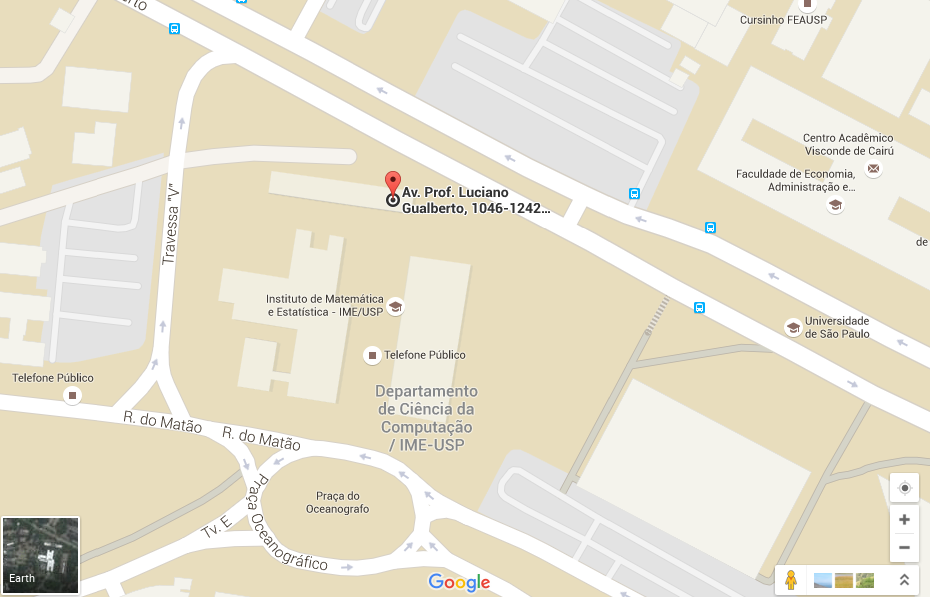
\includegraphics[height=100px]{ccsl-location}
        \end{figure}
        R. do Matão, 1010. Prédio do CCSL.
      \end{block}%
    \end{minipage}\hfill%
    \begin{minipage}[t][13em][t]{.3\textwidth}
      \begin{block}{\centering \large Inscrições pelo formulário}
        \center
        \begin{figure}[h]
          
\includegraphics[height=99px]{design_sprint_form_qr}
        \end{figure}
        \url{www.goo.gl/forms/xnOQVMfKoV}
      \end{block}
    \end{minipage}

    \vfill
    {\large Quaisquer dúvidas entre em contato por: mezurometrics@gmail.com}
  \end{centering}
\end{frame}
\end{document}
